\chapter{Diagonalization to solve vector differential equations}
In the last lecture, a second-order low-pass filter circuit using two resistors and two capacitors led us to the following differential equation:
\begin{align}
  \dod{}{t} \vec{x}
  &= A \vec{x} + \vec{b} u,
\end{align}
where \(\vec{x} = \begin{bmatrix}
  v_1(t) \\ v_2(t)
\end{bmatrix}\)
and \(\vec{x}(0)\) or \(\vec{x}(t_0)\) is known.
We represented \(\vec{x}\) as a linear combination of \(A\)'s eigenvectors \(\vec{v}_1\) (for eigenvalue \(\lambda_1\)) and \(\vec{v}_2\) (for eigenvalue \(\lambda_2\)):
\begin{align}
  \vec{x}
  &= \vec v_1 \tilde x_1
  + \vec v_2 \tilde x_2\\
  &=
  \begin{bmatrix}
    \vec v_1 & \vec v_2
  \end{bmatrix}
  \begin{bmatrix}
    \tilde x_1\\
    \tilde x_2
  \end{bmatrix}
    = V \vec {\tilde x}
\end{align}
We will assume that \(\lambda_1\) and \(\lambda_2\) are distinct, which implies that \(A\) has an invertible matrix of linearly independent eigenvectors \(V\).%
% \footnote{The proof of this fact is beyond the scope of this course.}
 We established that
\begin{align}
  A V &= V \Lambda, \quad
  V = \begin{bmatrix}
    \vec v_1 & \vec v_2
\end{bmatrix}, \quad
  \Lambda = \begin{bmatrix}
    \lambda_1 & 0 \\
    0 & \lambda 2
\end{bmatrix}.
\end{align}
These findings are summarized in \autoref{figure:lec6-diagonalization-commutative}, which shows how \(\vec x\), \(A \vec{x}\), \(\vec {\tilde x}\), and \(\Lambda \vec{\tilde x}\) are related by matrix multiplication (along arrows).

\begin{figure}
  \centering
  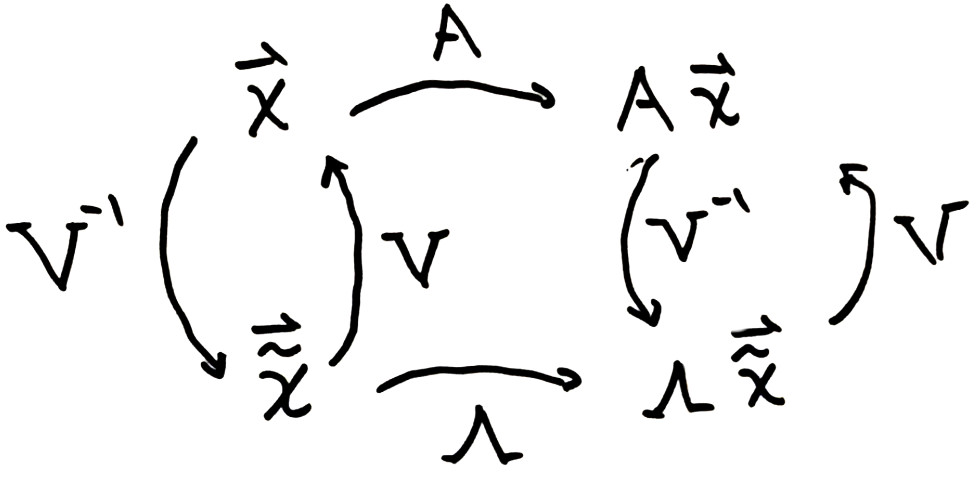
\includegraphics[width=0.75\linewidth]{figures/6/diagonalization-commutative}
  \caption{Illustration of multiplication actions of \(A\), \(\Lambda\), \(V\), and \(V^{-1}\).}
  \label{figure:lec6-diagonalization-commutative}
\end{figure}

\section{Solution technique}
A system
\begin{align}
  \dod{}{t} \vec x
  &= A \vec x + \vec b u; \quad \vec x (t_0)
\end{align}
is solved as follows:
\begin{enumerate}
  \item Compute eigenvalues \(\lambda_1\) and \(\lambda_2\) of \(A\), as well as their respective eigenvectors \(\vec v_1\) and \(\vec v_2\).
  \item Construct \(V = \begin{bmatrix}
            \vec v_1 & \vec v_2
        \end{bmatrix}\)
        and define
        \(\vec{\tilde x} = V^{-1} x\).
  \item
  Construct \(\Lambda = \begin{bmatrix}
    \lambda_1 & 0 \\
    0 & \lambda_2
  \end{bmatrix}\) and \(\tilde b = V^{-1} b\).
  Solve the differential equation
  \(\dod{}{t} \vec{\tilde x} = \Lambda \vec{\tilde x} + \tilde b u\)
  with initial condition \(\tilde x(t_0) = V^{-1} x(t_0)\). (More on this later.)
  \item Recover a solution for \(\vec x\) using \(\vec x = V \vec{\tilde x}\).
\end{enumerate}

\section{Numerical example from RCRC circuit}
\autoref{eq:lec5-RCRC-numerical} captured a second-order low-pass filter using
\begin{align}
  A = \begin{bmatrix}
    -5 & \phantom{-}2 \\ \phantom{-}2 & -2
\end{bmatrix} \quad \text{and} \quad
  \vec b = \begin{bmatrix}
    3 \\ 0
\end{bmatrix}.
\end{align}
We will solve the differential equation for \(\vec x = \begin{bmatrix}
  v_1 \\ v_2
\end{bmatrix}\) using the technique of the previous section.

\subsection{Eigenvalues and eigenvectors}
We will solve for eigenvectors \(\lambda\) as roots of \(\det\del{\lambda I - A}\), the characteristic polynomial of \(A\).
\begin{align}
  \det
  \begin{bmatrix}
    \lambda + 5 & -2 \\
    -2 & \lambda + 2
  \end{bmatrix}
  &= \lambda^2 + 7\lambda + 6 = 0\\
  \intertext{This quadratic equation in the indeterminate \(\lambda\) is called the \emph{characteristic equation} of \(A\).
  It has the following roots:}
  \lambda_1 &= -1; \quad \lambda_2 = -6.
  \intertext{Next we will solve for an eigenvector belonging to eigenvalue \(\lambda_1\), by choosing a nonzero vector from the null space of \(\lambda_1I - A\):}
  \lambda_1 I - A &= \begin{bmatrix}
    \phantom{-}4 & -2 \\
    -2 & \phantom{-}1
  \end{bmatrix}\\
  \vec v_1 &= \begin{bmatrix}
    1 \\ 2
  \end{bmatrix}
  \intertext{\ldots and, \emph{mutatis mutandis}, for \(\lambda_2\):}
  \lambda_2 I - A &= \begin{bmatrix}
    -1 & -2 \\
    -2 & -4
  \end{bmatrix}\\
  \vec v_2 &= \begin{bmatrix}
    \phantom{-}2 \\ -1
  \end{bmatrix}
\end{align}

\subsection{Differential equation in new coordinates}
In our example,
\begin{align}
  V &= \begin{bmatrix}
    1 & 2 \\
    2 & -1
\end{bmatrix}, \quad \text{so}\\
V^{-1} &= \begin{bmatrix}
  \frac{1}{5} & \frac{2}{5} \\[3pt]
  \frac{2}{5} & -\frac{1}{5}
\end{bmatrix}.
\intertext{
Our differential equation in \(\vec{\tilde x}\) will be
}
\dod{}{t} \vec{\tilde x}
&= \Lambda \vec{\tilde x} + V^{-1} \vec b u\\
&= \begin{bmatrix}
  -1 & \phantom{-}0 \\
  \phantom{-}0 & -6
\end{bmatrix}
\vec{\tilde x}
+ \begin{bmatrix}
  \frac{3}{5} \\[3pt] \frac{6}{5}
\end{bmatrix}.
\intertext{
   With \(t_0 = 0\), \(\vec {\tilde x}\) is solved as follows:
}
\vec{\tilde x} (t)
&= \del{\text{homogeneous solution}} + \del{\text{particular solution}}\\
&= \begin{bmatrix}
  e^{\lambda_1 t} & 0\\
  0 & e^{\lambda_2 t}
\end{bmatrix}
\vec{\tilde x} (0)
+ \int_{0}^t
\begin{bmatrix}
  e^{\lambda_1(t - \tau)} & 0 \\
  0 & e^{\lambda_2(t - \tau)}
\end{bmatrix}
\vec{\tilde b}
u(\tau)
\dif \tau,
\end{align}
viz., in individual components,
\begin{align}
  \begin{cases}
  \tilde x_1 (t)
  = e^{\lambda_1 t} \tilde x_1(0) + \int_{0}^t e^{\lambda_1(t - \tau)}
    \tilde b_1 u(\tau) \dif \tau\\[3pt]
  \tilde x_2 (t)
  = e^{\lambda_2 t} \tilde x_2(0) + \int_{0}^t e^{\lambda_2(t - \tau)}
    \tilde b_2 u(\tau) \dif \tau
\end{cases}
\end{align}

\subsection{Solution in original coordinates}
A solution for \(\vec x(t)\) may be reconstituted from eigenbasis-aligned coordinates using the following equation:
\begin{align}
  \vec x(t)
  &= \begin{bmatrix}
    \vec v_1 & \vec v_2
\end{bmatrix}
\begin{bmatrix}
  \tilde x_1 (t) \\
  \tilde x_2 (t)
\end{bmatrix}.
\end{align}

\section{Introduction to inductors}
\begin{figure}
  \centering
  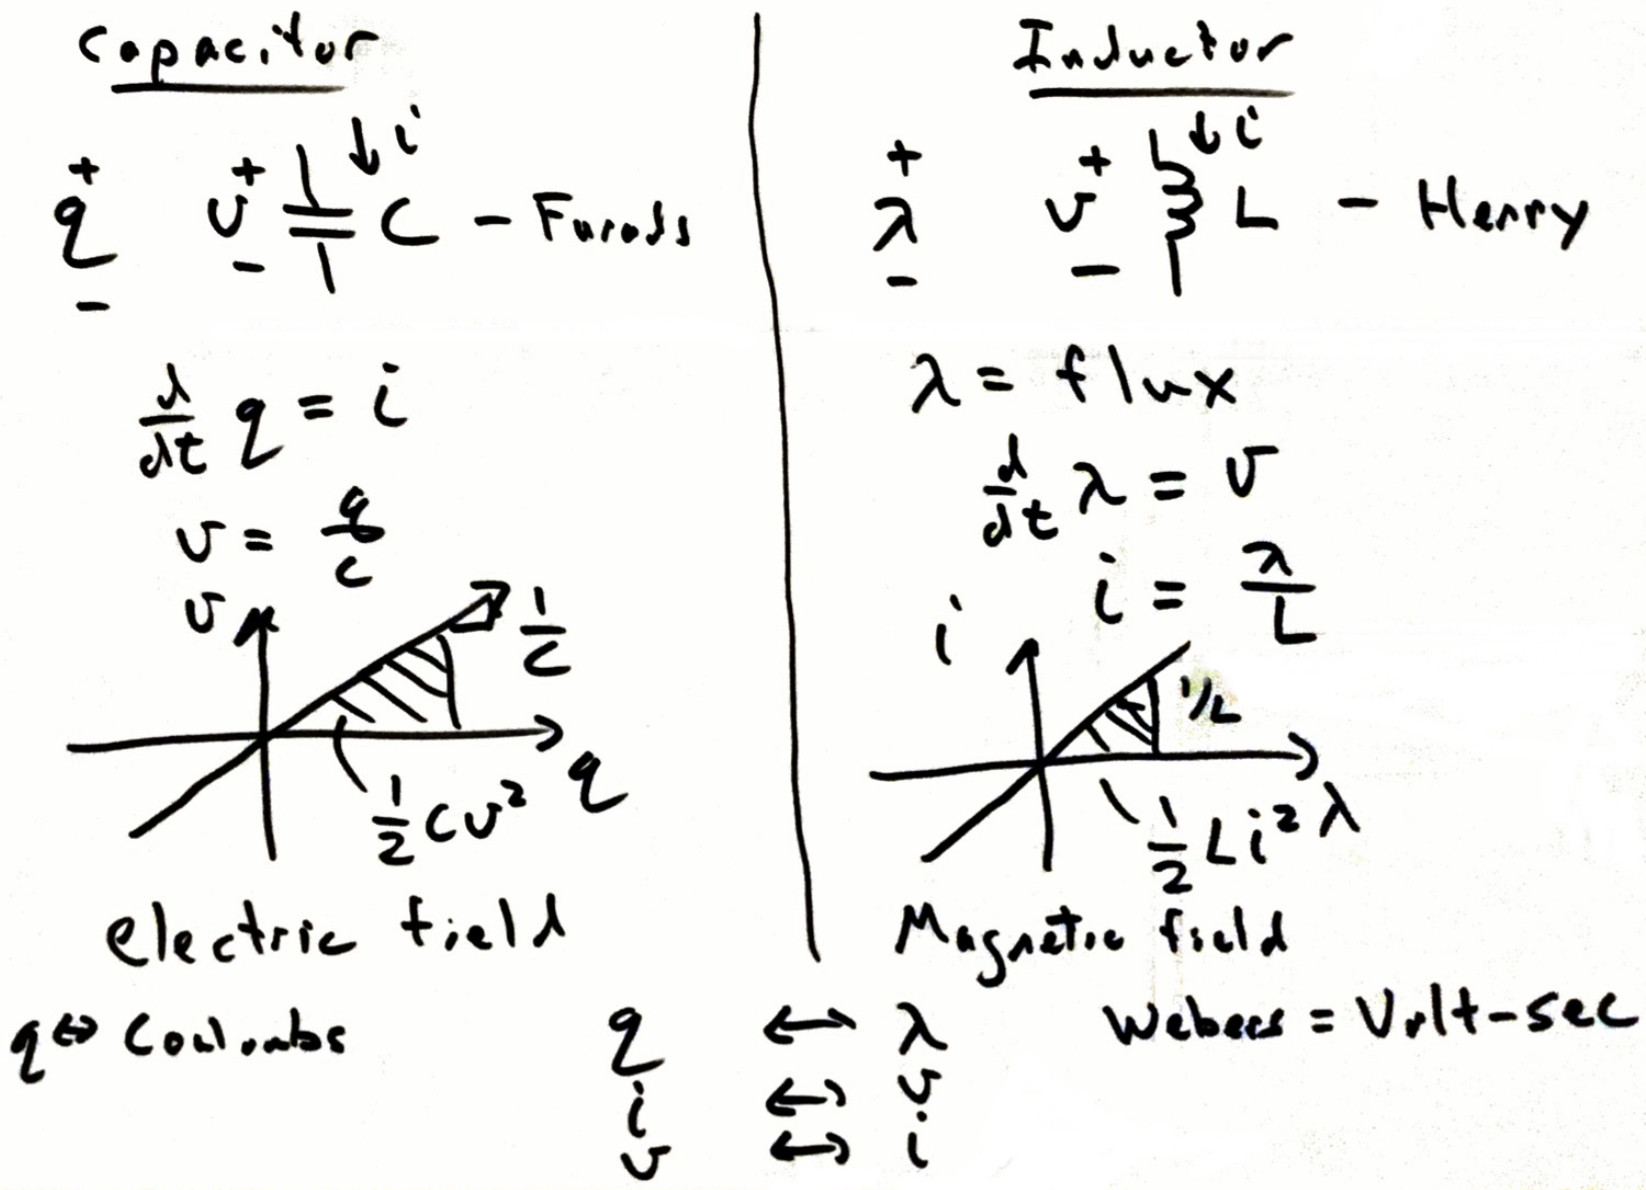
\includegraphics[width=1\linewidth]{figures/6/cap-vs-ind}
  \caption{Parallels between capacitors and inductors.}
  \label{figure:lec6-cap-vs-ind}
\end{figure}
Inductors are a branch element that are analogous to capacitors.
\autoref{figure:lec6-cap-vs-ind} compares them with capacitors,
and the parallels are repeated below.
\begin{align}
  q &= \text{charge (Coulomb)}
  & \lambda &= \text{flux (Weber = Volt-second)}\\
  \dod{}{t} q &= i & \dod{}{t} \lambda &= v\\
  v &= \frac{q}{C} & i &= \frac{\lambda}{L} \\
  E_{C} &= \frac{1}{2} Cv^2 & E_{L} &= \frac{1}{2} Li^2
\end{align}

\section{Example: RL circuit}
\begin{figure}
  \centering
  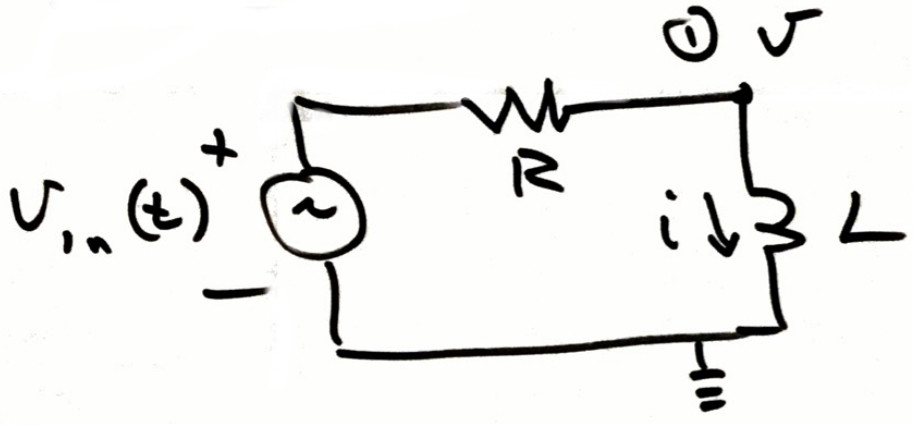
\includegraphics[width=0.75\linewidth]{figures/6/RL}
  \caption{RL circuit, which is similar to an RC circuit (cf.~\autoref{figure:lec4-RC}).}
  \label{figure:lec6-RL}
\end{figure}
\autoref{figure:lec6-RL}
shows a circuit with a time-varying voltage source, a resistor, and an inductor.
KCL at the marked upper right node yields
\begin{align}
  \frac{v - v_\text{in}}{R} + i &= 0.
  \intertext{In addition, from the current-voltage relationship of an inductor,}
  L \dod{}{t} i &= v.
  \intertext{Eliminating \(v\) and isolating \(\dod{}{t} i\), we have}
  \dod{}{t}i &= -\frac{R}{L} i + \frac{v_\text{in}}{L}.
\end{align}
The state variable for an inductor is \(i\), and this differential equation may be solved the same way we solved RC circuits.
